\documentclass[11pt,a4paper]{article}
\usepackage[utf8]{inputenc}
\usepackage{amsmath,amsfonts,amssymb}
\usepackage{graphicx}
\usepackage{geometry}
\geometry{margin=1in}
\usepackage{booktabs}
\usepackage{hyperref}
\usepackage{float}
\usepackage{tikz}
\usetikzlibrary{shapes,arrows,positioning}

\title{\textbf{EE3621: Digital Signal Processing} \\ \Large Lecture 1: Course Introduction \& Discrete-Time Signals \\ \large (III B.Tech EEE)}
\author{Lecture Notes (40-Minute Plan)}
\date{}

\usepackage{xcolor}
\definecolor{darkbg}{HTML}{0d121f}
\definecolor{lighttext}{HTML}{e2e8f0}
\definecolor{primary}{HTML}{8b5cf6}
\definecolor{secondary}{HTML}{0dd5c5}

\pagecolor{darkbg}
\color{lighttext}

\hypersetup{
    colorlinks=true,
    linkcolor=secondary,
    urlcolor=secondary
}

\begin{document}

\maketitle

\section{Lecture Plan \& Objectives (40 Minutes Breakdown)}
\begin{itemize}
    \item \textbf{00:00 -- 05:00 (5 mins):} Welcome, Course Objectives, \& Syllabus Walkthrough
    \item \textbf{05:00 -- 18:00 (13 mins):} Introduction to DSP, Analog vs. Digital Processing (Block Diagram, Pros \& Cons)
    \item \textbf{18:00 -- 30:00 (12 mins):} Classification of Discrete-Time (DT) Signals (Periodicity, Energy/Power, Symmetry)
    \item \textbf{30:00 -- 38:00 (8 mins):} Elementary Sequences (Impulse, Step, Ramp, Sinusoid, Exponential)
    \item \textbf{38:00 -- 40:00 (2 mins):} Q\&A and Summary
\end{itemize}

\noindent\rule{\textwidth}{0.5pt}

\section{Introduction to DSP \& Analog vs. Digital Processing}

A \textbf{signal} is any physical quantity that varies with time, space, or any other independent variable, carrying information. In electrical engineering, examples include voltage waveforms $v(t)$, alternating current $i(t)$, and power grid frequency.

\begin{itemize}
    \item \textbf{Analog Signal Processing (ASP):} Signals are processed in their continuous-time, continuous-amplitude form using analog hardware such as resistors ($R$), inductors ($L$), capacitors ($C$), and operational amplifiers.
    \item \textbf{Digital Signal Processing (DSP):} Signals are represented as sequences of numbers (discrete-time, quantized amplitude) and processed using digital processors (microprocessors, FPGAs, or DSP chips).
\end{itemize}

\subsection{Typical DSP System Block Diagram}
An analog input signal $x(t)$ is first converted to a digital sequence, processed mathematically, and then optionally converted back to analog:

\begin{figure}[H]
\centering
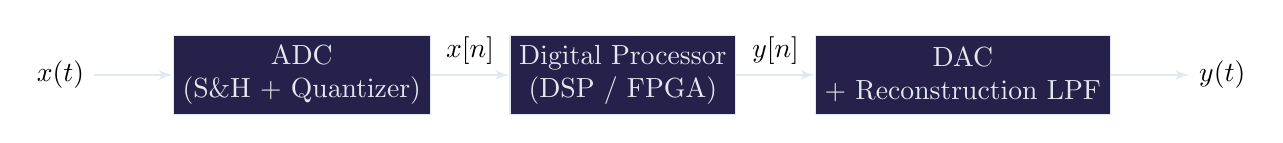
\begin{tikzpicture}[
    block/.style={draw=lighttext, rectangle, minimum height=1cm, minimum width=2cm, align=center, fill=primary!20!darkbg, text=lighttext},
    line/.style={draw=lighttext, -latex', thick}
]
    \node (input) {$x(t)$};
    \node [block, right=1cm of input] (adc) {ADC\\(S\&H + Quantizer)};
    \node [block, right=1cm of adc] (dsp) {Digital Processor\\(DSP / FPGA)};
    \node [block, right=1cm of dsp] (dac) {DAC\\+ Reconstruction LPF};
    \node [right=1cm of dac] (output) {$y(t)$};
    
    \path [line] (input) -- (adc);
    \path [line] (adc) -- node[above] {$x[n]$} (dsp);
    \path [line] (dsp) -- node[above] {$y[n]$} (dac);
    \path [line] (dac) -- (output);
\end{tikzpicture}
\caption{Block diagram of a typical real-time DSP system.}
\label{fig:dsp_block_diagram}
\end{figure}

\subsection{ASP vs. DSP Comparison}
\begin{table}[H]
\centering
\begin{tabular}{p{3.5cm} p{5.5cm} p{5.5cm}}
\toprule
\textbf{Feature} & \textbf{Analog Signal Processing (ASP)} & \textbf{Digital Signal Processing (DSP)} \\
\midrule
\textbf{Components} & Resistors, inductors, capacitors, Op-Amps. & Multipliers, adders, registers, software. \\
\textbf{Accuracy} & Limited by component tolerances (e.g., $\pm 5\%$) and drift. & Highly accurate; limited only by word-length. \\
\textbf{Flexibility} & Hard to modify; requires physical design changes. & Extremely flexible; simple software updates. \\
\textbf{Storage} & Hard to store without degradation. & Easy storage on flash/digital media. \\
\textbf{Speed} & Works at very high frequencies (real-time). & Limited by sampling rate and clock speed. \\
\bottomrule
\end{tabular}
\caption{Comparison of ASP and DSP.}
\label{tab:comparison}
\end{table}

\subsection{Analog Pre-Processing: AAF and S\&H Circuits}
Before an analog signal can be sampled and digitized, it must pass through two physical analog circuits:
\begin{enumerate}
    \item \textbf{Anti-Aliasing Filter (AAF):} This is typically a passive or active RC low-pass filter. It attenuates frequency components above the Nyquist frequency $f_N = f_s/2$. The RC cutoff frequency $f_c$ must satisfy:
    \begin{equation}
    f_c = \frac{1}{2\pi R C} \le \frac{f_s}{2} \implies R C \ge \frac{1}{\pi f_s}
    \end{equation}
    If this condition is violated, out-of-band noise folds back into the passband, causing aliasing.
    
    \item \textbf{Sample-and-Hold (S\&H) Circuit:} This circuit captures the continuous analog voltage and holds it steady for quantization. It consists of a MOSFET switch with on-resistance $R_{on}$, a hold capacitor $C_{hold}$, and an op-amp buffer.
    \begin{itemize}
        \item \textbf{Tracking Mode:} Switch is closed. The capacitor charges with time constant $\tau_{acq} = R_{on} C_{hold}$. To achieve $0.1\%$ accuracy (for a 10-bit ADC), the tracking time $T_{track}$ must be:
        \begin{equation}
        T_{track} \ge 7 \tau_{acq} = 7 R_{on} C_{hold}
        \end{equation}
        \item \textbf{Hold Mode:} Switch is open. The capacitor discharges through the buffer input resistance $R_{in}$ with time constant $\tau_{hold} = R_{in} C_{hold}$. To prevent signal voltage decay (droop), we require:
        \begin{equation}
        R_{in} C_{hold} \gg T_s = \frac{1}{f_s}
        \end{equation}
    \end{itemize}
\end{enumerate}

\subsection{Visualizing Signal Types}
To understand the transformation of a signal through a DSP system, we can observe the difference between an analog signal, a sampled (discrete-time) signal, and a digital (quantized) signal.

\begin{figure}[H]
\centering
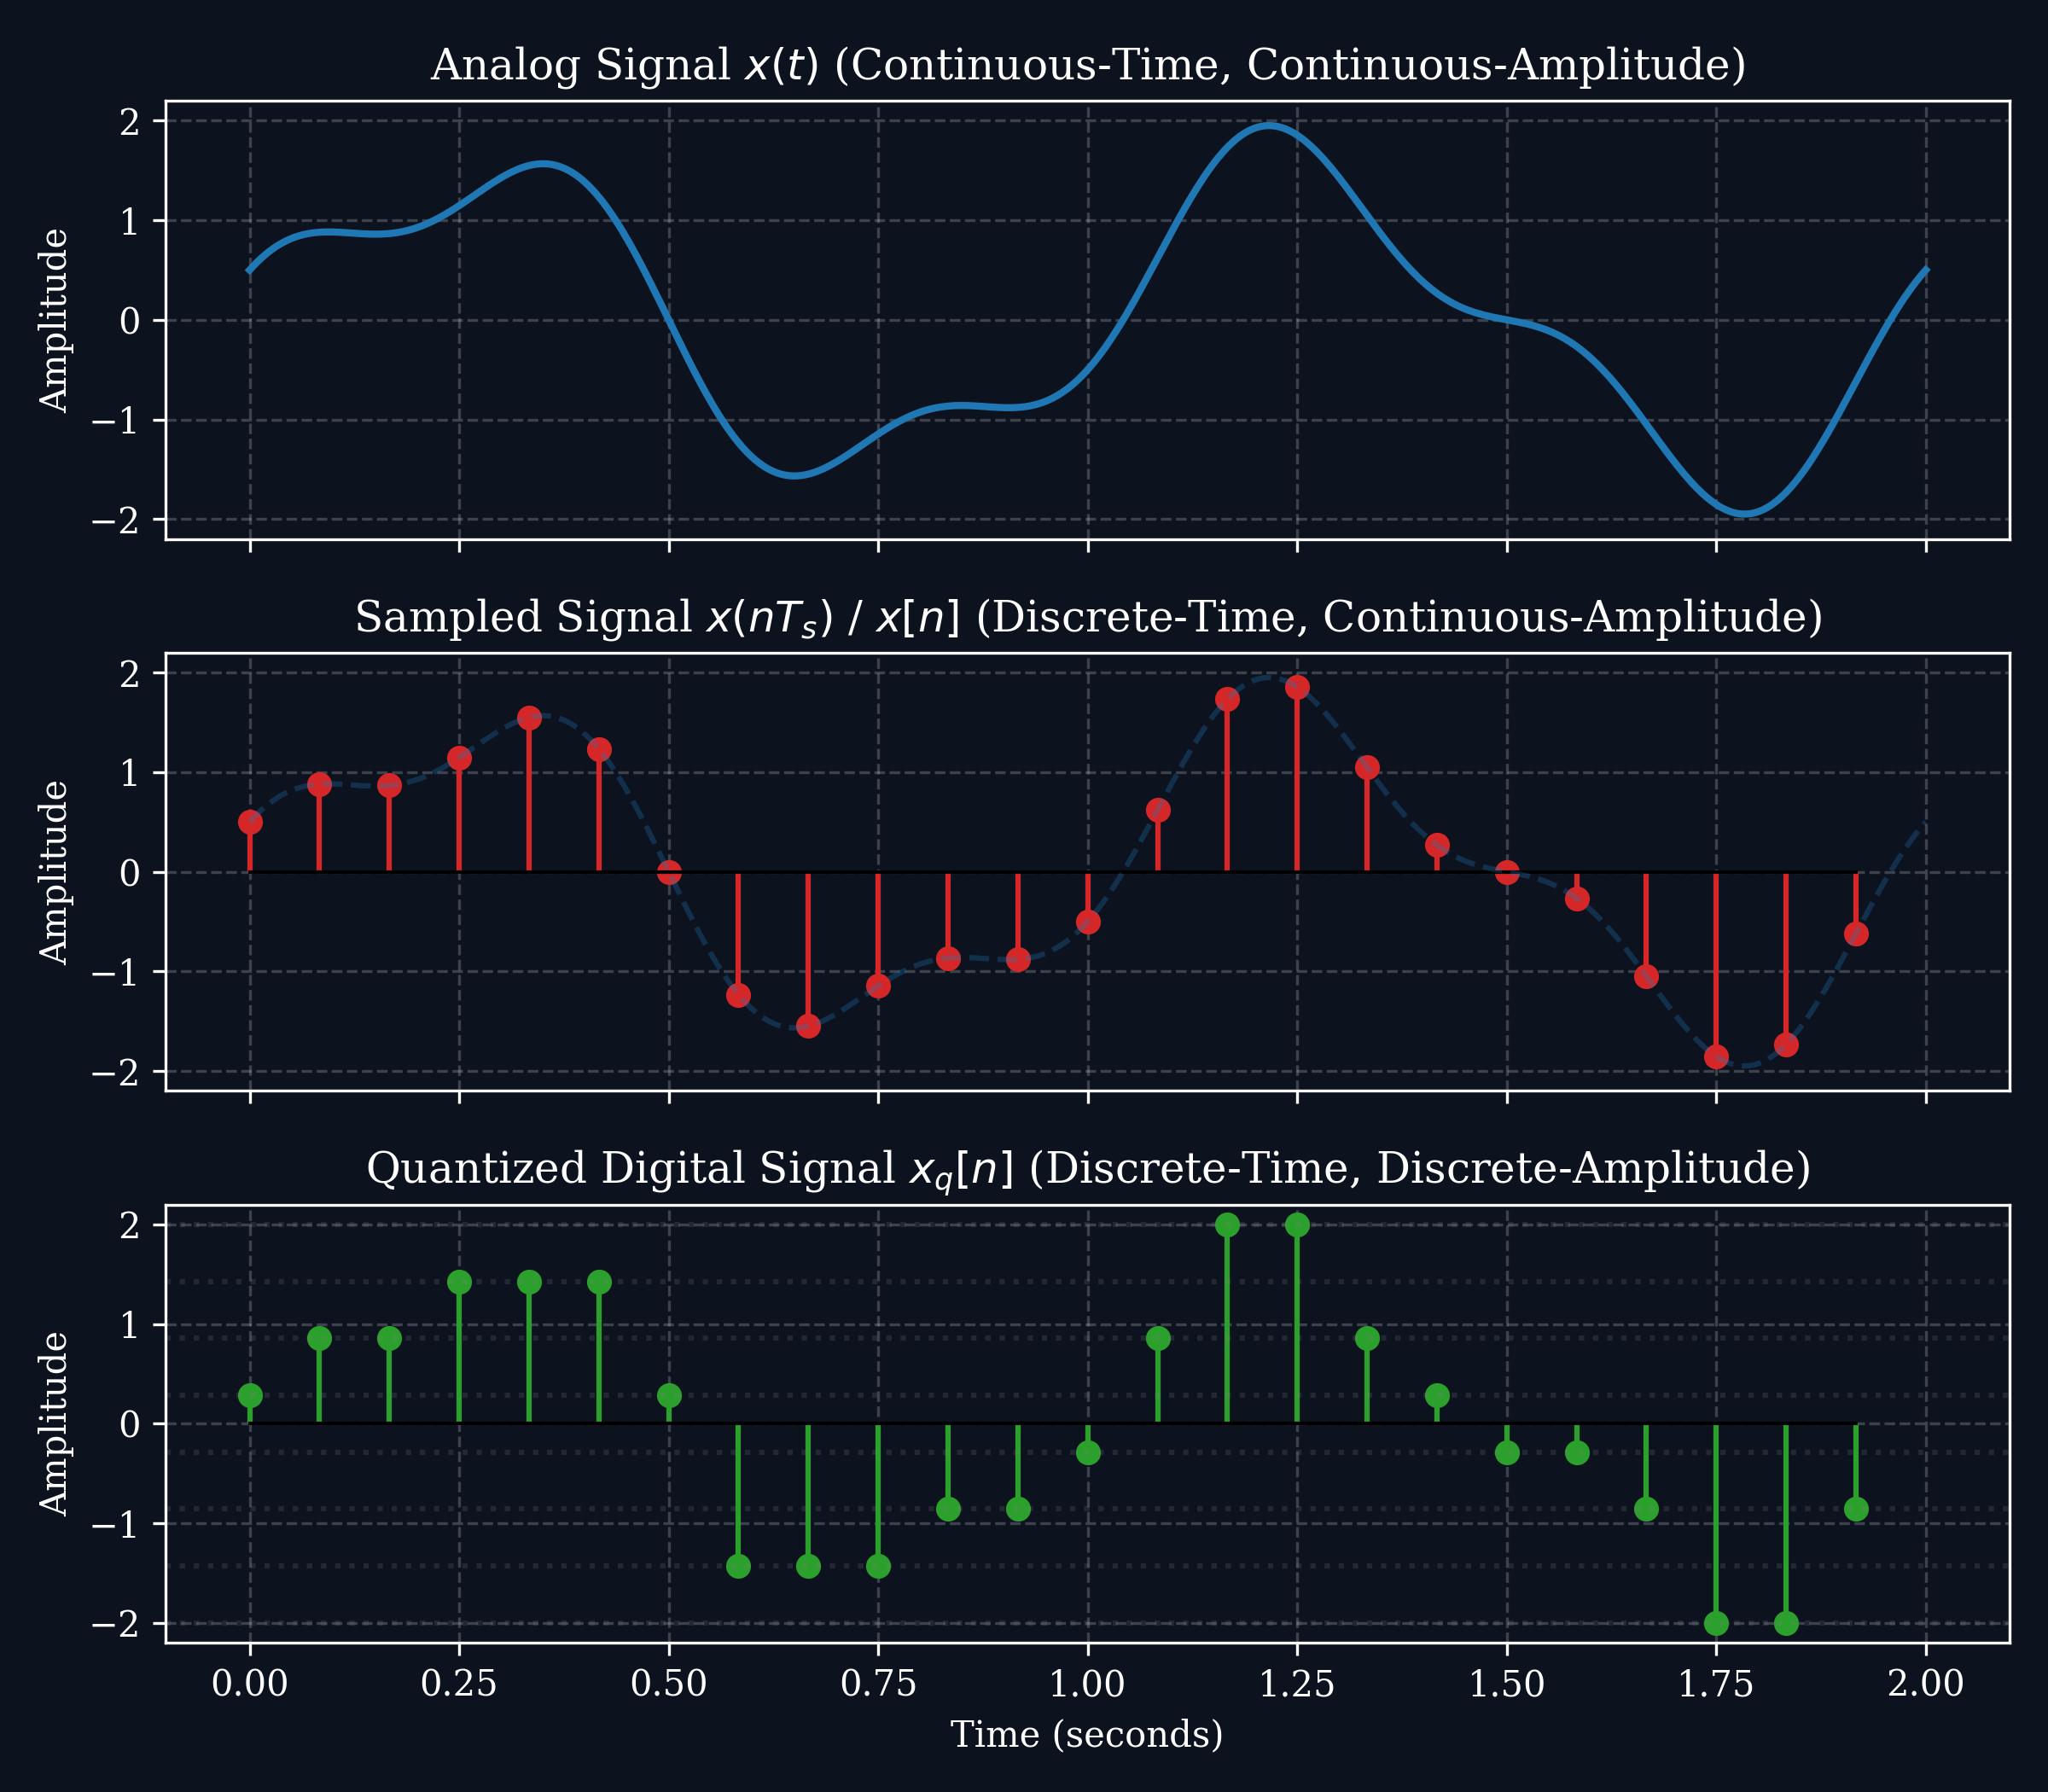
\includegraphics[width=0.85\textwidth]{images/analog_vs_digital.png}
\caption{Analog signal $x(t)$, sampled sequence $x[n]$, and quantized digital sequence $x_q[n]$.}
\label{fig:analog_vs_digital}
\end{figure}

\subsection{Quantization Resolution and Bit Depth}
Quantization is the process of converting a continuous-amplitude signal into a discrete-amplitude signal by mapping each continuous value to the nearest discrete level. The resolution of a quantizer depends on the number of bits, $B$:
\begin{itemize}
    \item \textbf{Quantization Levels ($L$):} The number of discrete amplitude steps available:
    \begin{equation}
    L = 2^B
    \end{equation}
    \item \textbf{Step Size ($\Delta$):} The amplitude difference between adjacent levels for a full-scale range $R$ (from $-V_{ref}$ to $+V_{ref}$):
    \begin{equation}
    \Delta = \frac{R}{2^B}
    \end{equation}
    \item \textbf{Quantization Noise:} The rounding error $e[n] = x_q[n] - x[n]$ is bounded by $-\Delta/2 \le e[n] \le \Delta/2$. Under uniform assumptions, the average noise power is:
    \begin{equation}
    \sigma_e^2 = \frac{\Delta^2}{12}
    \end{equation}
    \item \textbf{Signal-to-Quantization-Noise Ratio (SQNR):} For a full-scale sinusoidal input, the SQNR is:
    \begin{equation}
    \text{SQNR (dB)} \approx 6.02 B + 1.76 \text{ dB}
    \end{equation}
    This implies that each additional bit of resolution increases the SQNR by approximately $6\text{ dB}$, representing a significant reduction in noise power and stored data fidelity.
\end{itemize}

\section{Discrete-Time (DT) Signals \& Classification}
A discrete-time signal $x[n]$ is defined only at integer values of the independent variable $n$ (sample index). Mathematically, it is a sequence of numbers:
\begin{equation}
x[n] = \{x[-1], \underline{x[0]}, x[1], x[2], \dots\}
\end{equation}

\subsection{Key Classifications}
\begin{enumerate}
    \item \textbf{Periodic vs. Aperiodic:} A signal $x[n]$ is periodic if there exists an integer $N > 0$ such that $x[n+N] = x[n]$ for all $n$. For a sinusoidal signal $A\cos(\omega_0 n)$, it is periodic only if:
    \begin{equation}
    \frac{\omega_0}{2\pi} = \frac{m}{N} \quad \text{where } m, N \in \mathbb{Z}
    \end{equation}
    If the frequency ratio is irrational, the signal is aperiodic.
    
    \item \textbf{Even vs. Odd Symmetry:}
    \begin{itemize}
        \item Even: $x[-n] = x[n]$ (Symmetrical about the y-axis).
        \item Odd: $x[-n] = -x[n]$ (Antisymmetrical; implies $x[0] = 0$).
    \end{itemize}
    \begin{figure}[H]
    \centering
    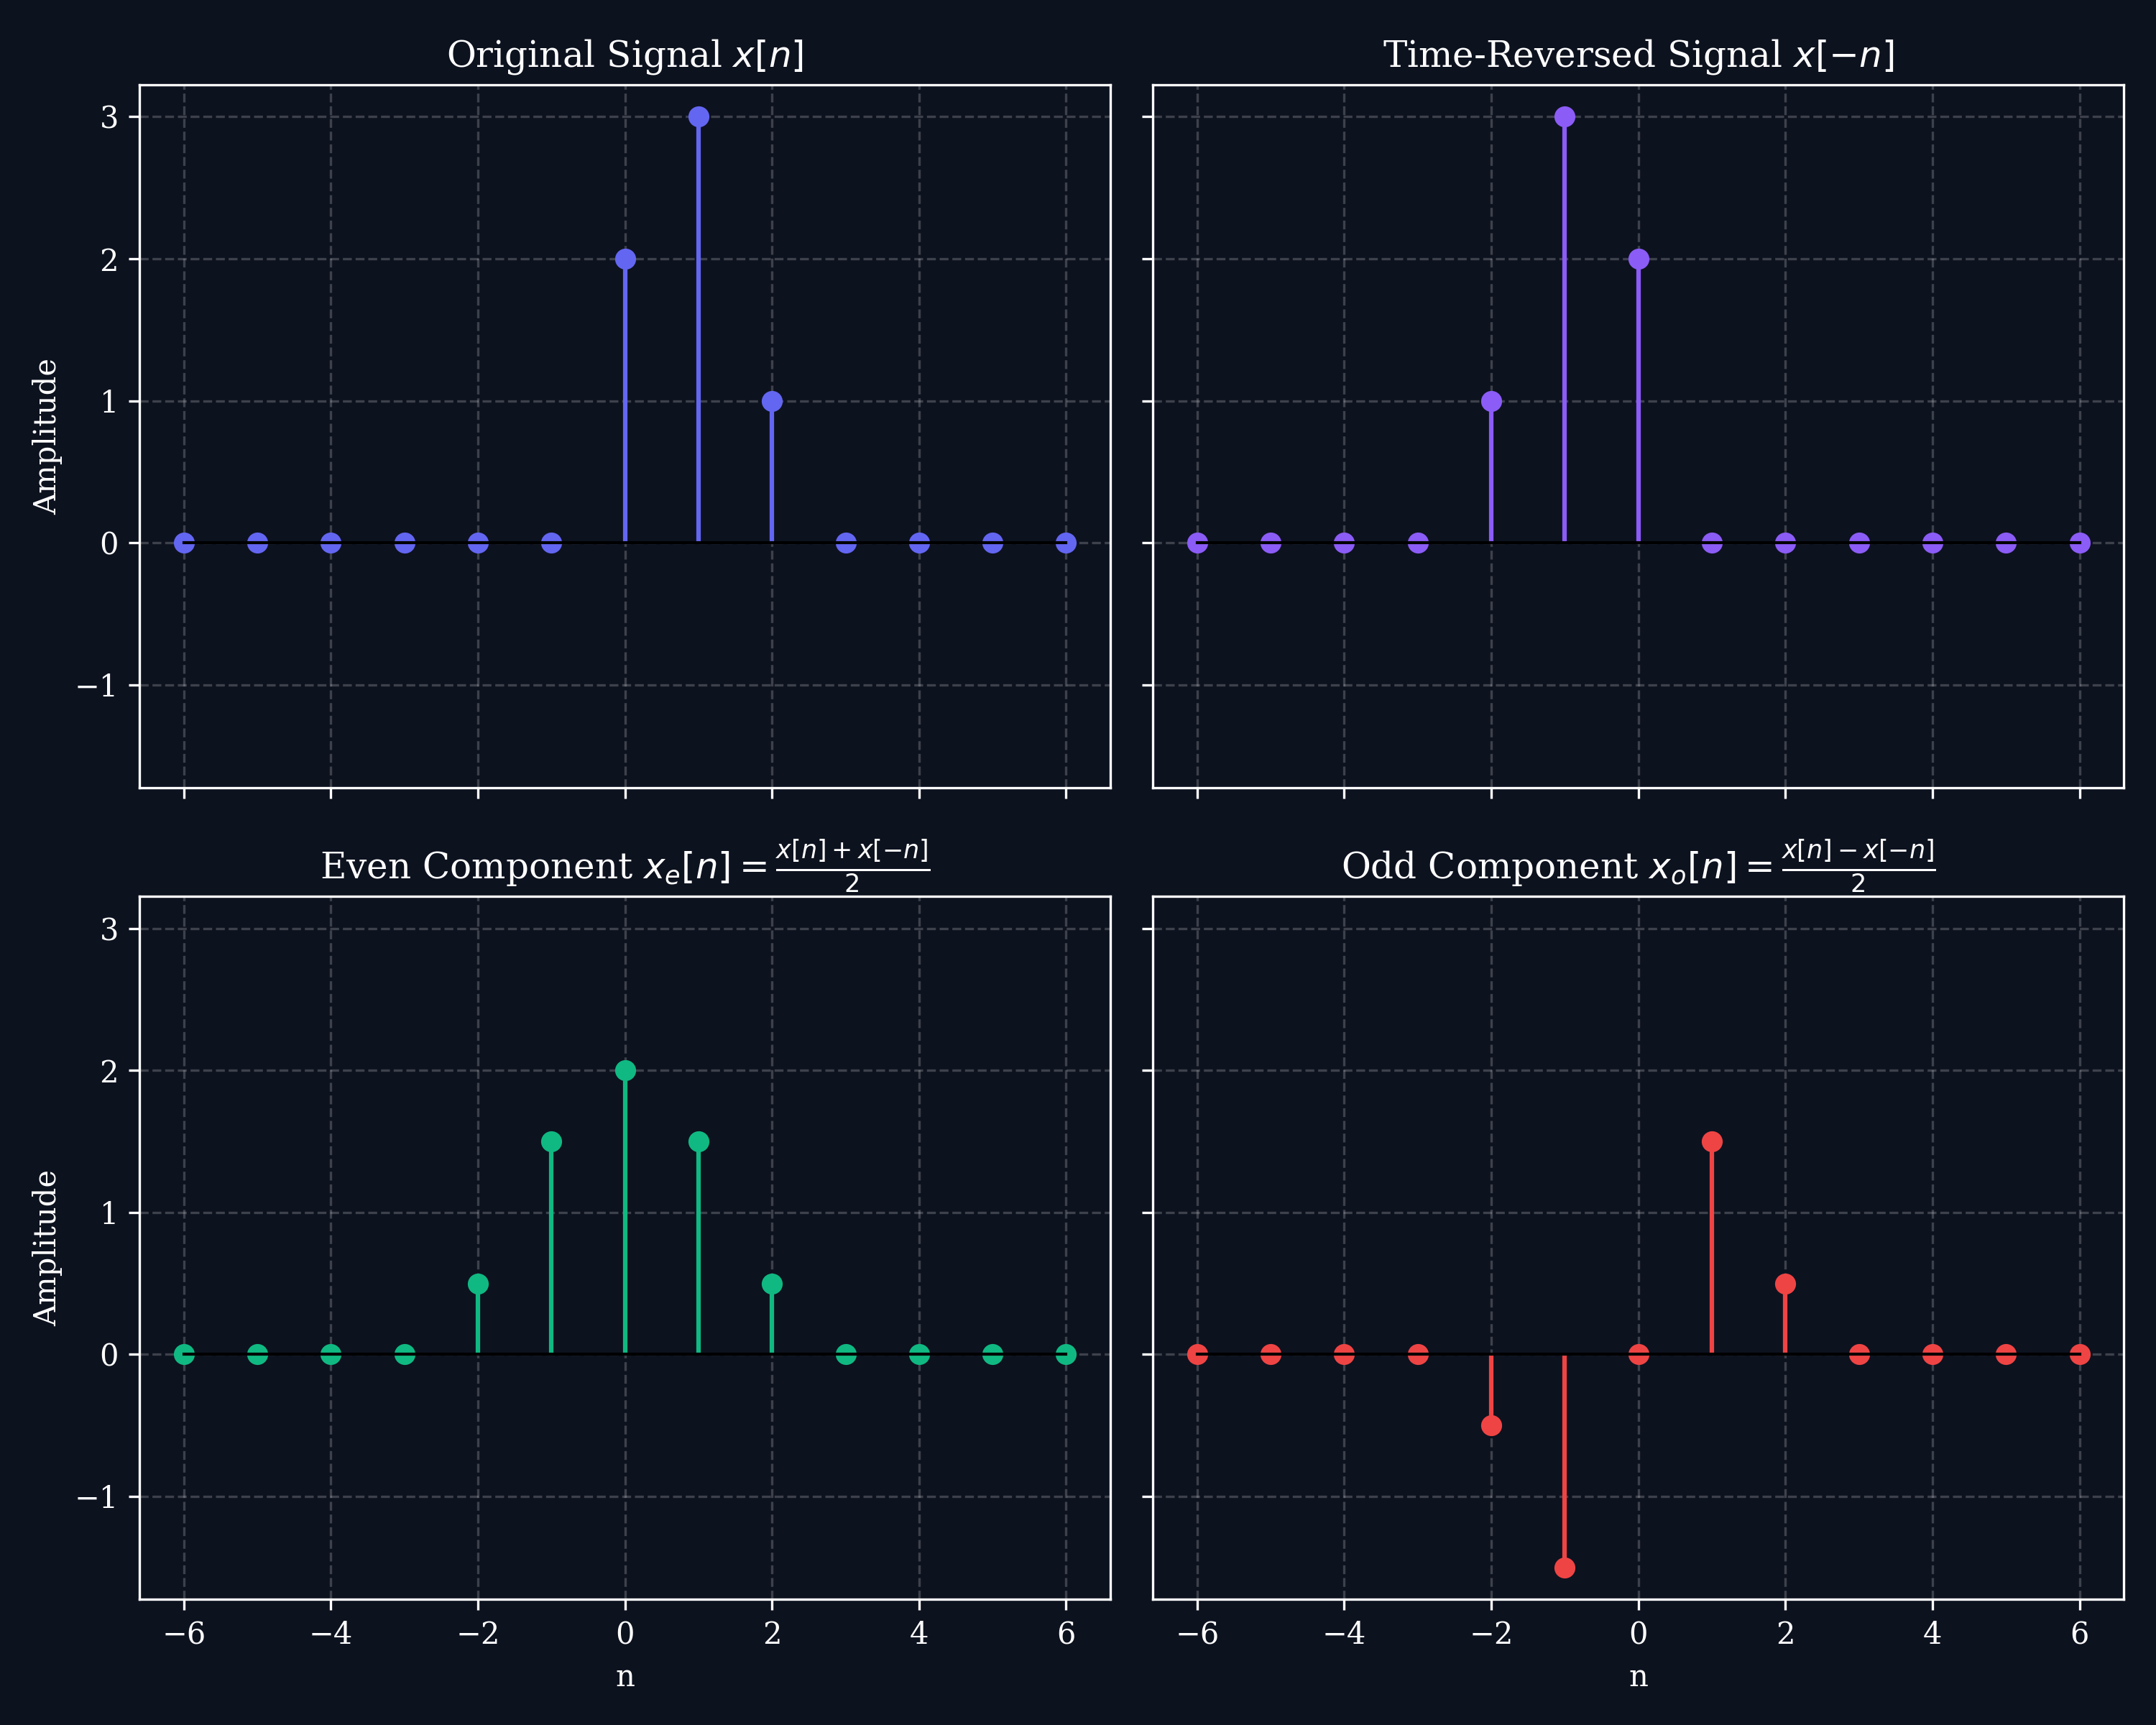
\includegraphics[width=0.75\textwidth]{images/even_odd_decomposition.png}
    \caption{Decomposition of an asymmetric sequence $x[n]$ into its even component $x_e[n]$ and odd component $x_o[n]$.}
    \label{fig:even_odd_decomp}
    \end{figure}
    
    \item \textbf{Energy vs. Power:}
    \begin{itemize}
        \item Total Energy: $E = \sum_{n=-\infty}^{\infty} |x[n]|^2$.
        \item Average Power: $P = \lim_{N \to \infty} \frac{1}{2N+1} \sum_{n=-N}^{N} |x[n]|^2$.
        \item Energy Signal: $0 < E < \infty \implies P = 0$.
        \item Power Signal: $0 < P < \infty \implies E = \infty$.
    \end{itemize}
    \begin{figure}[H]
    \centering
    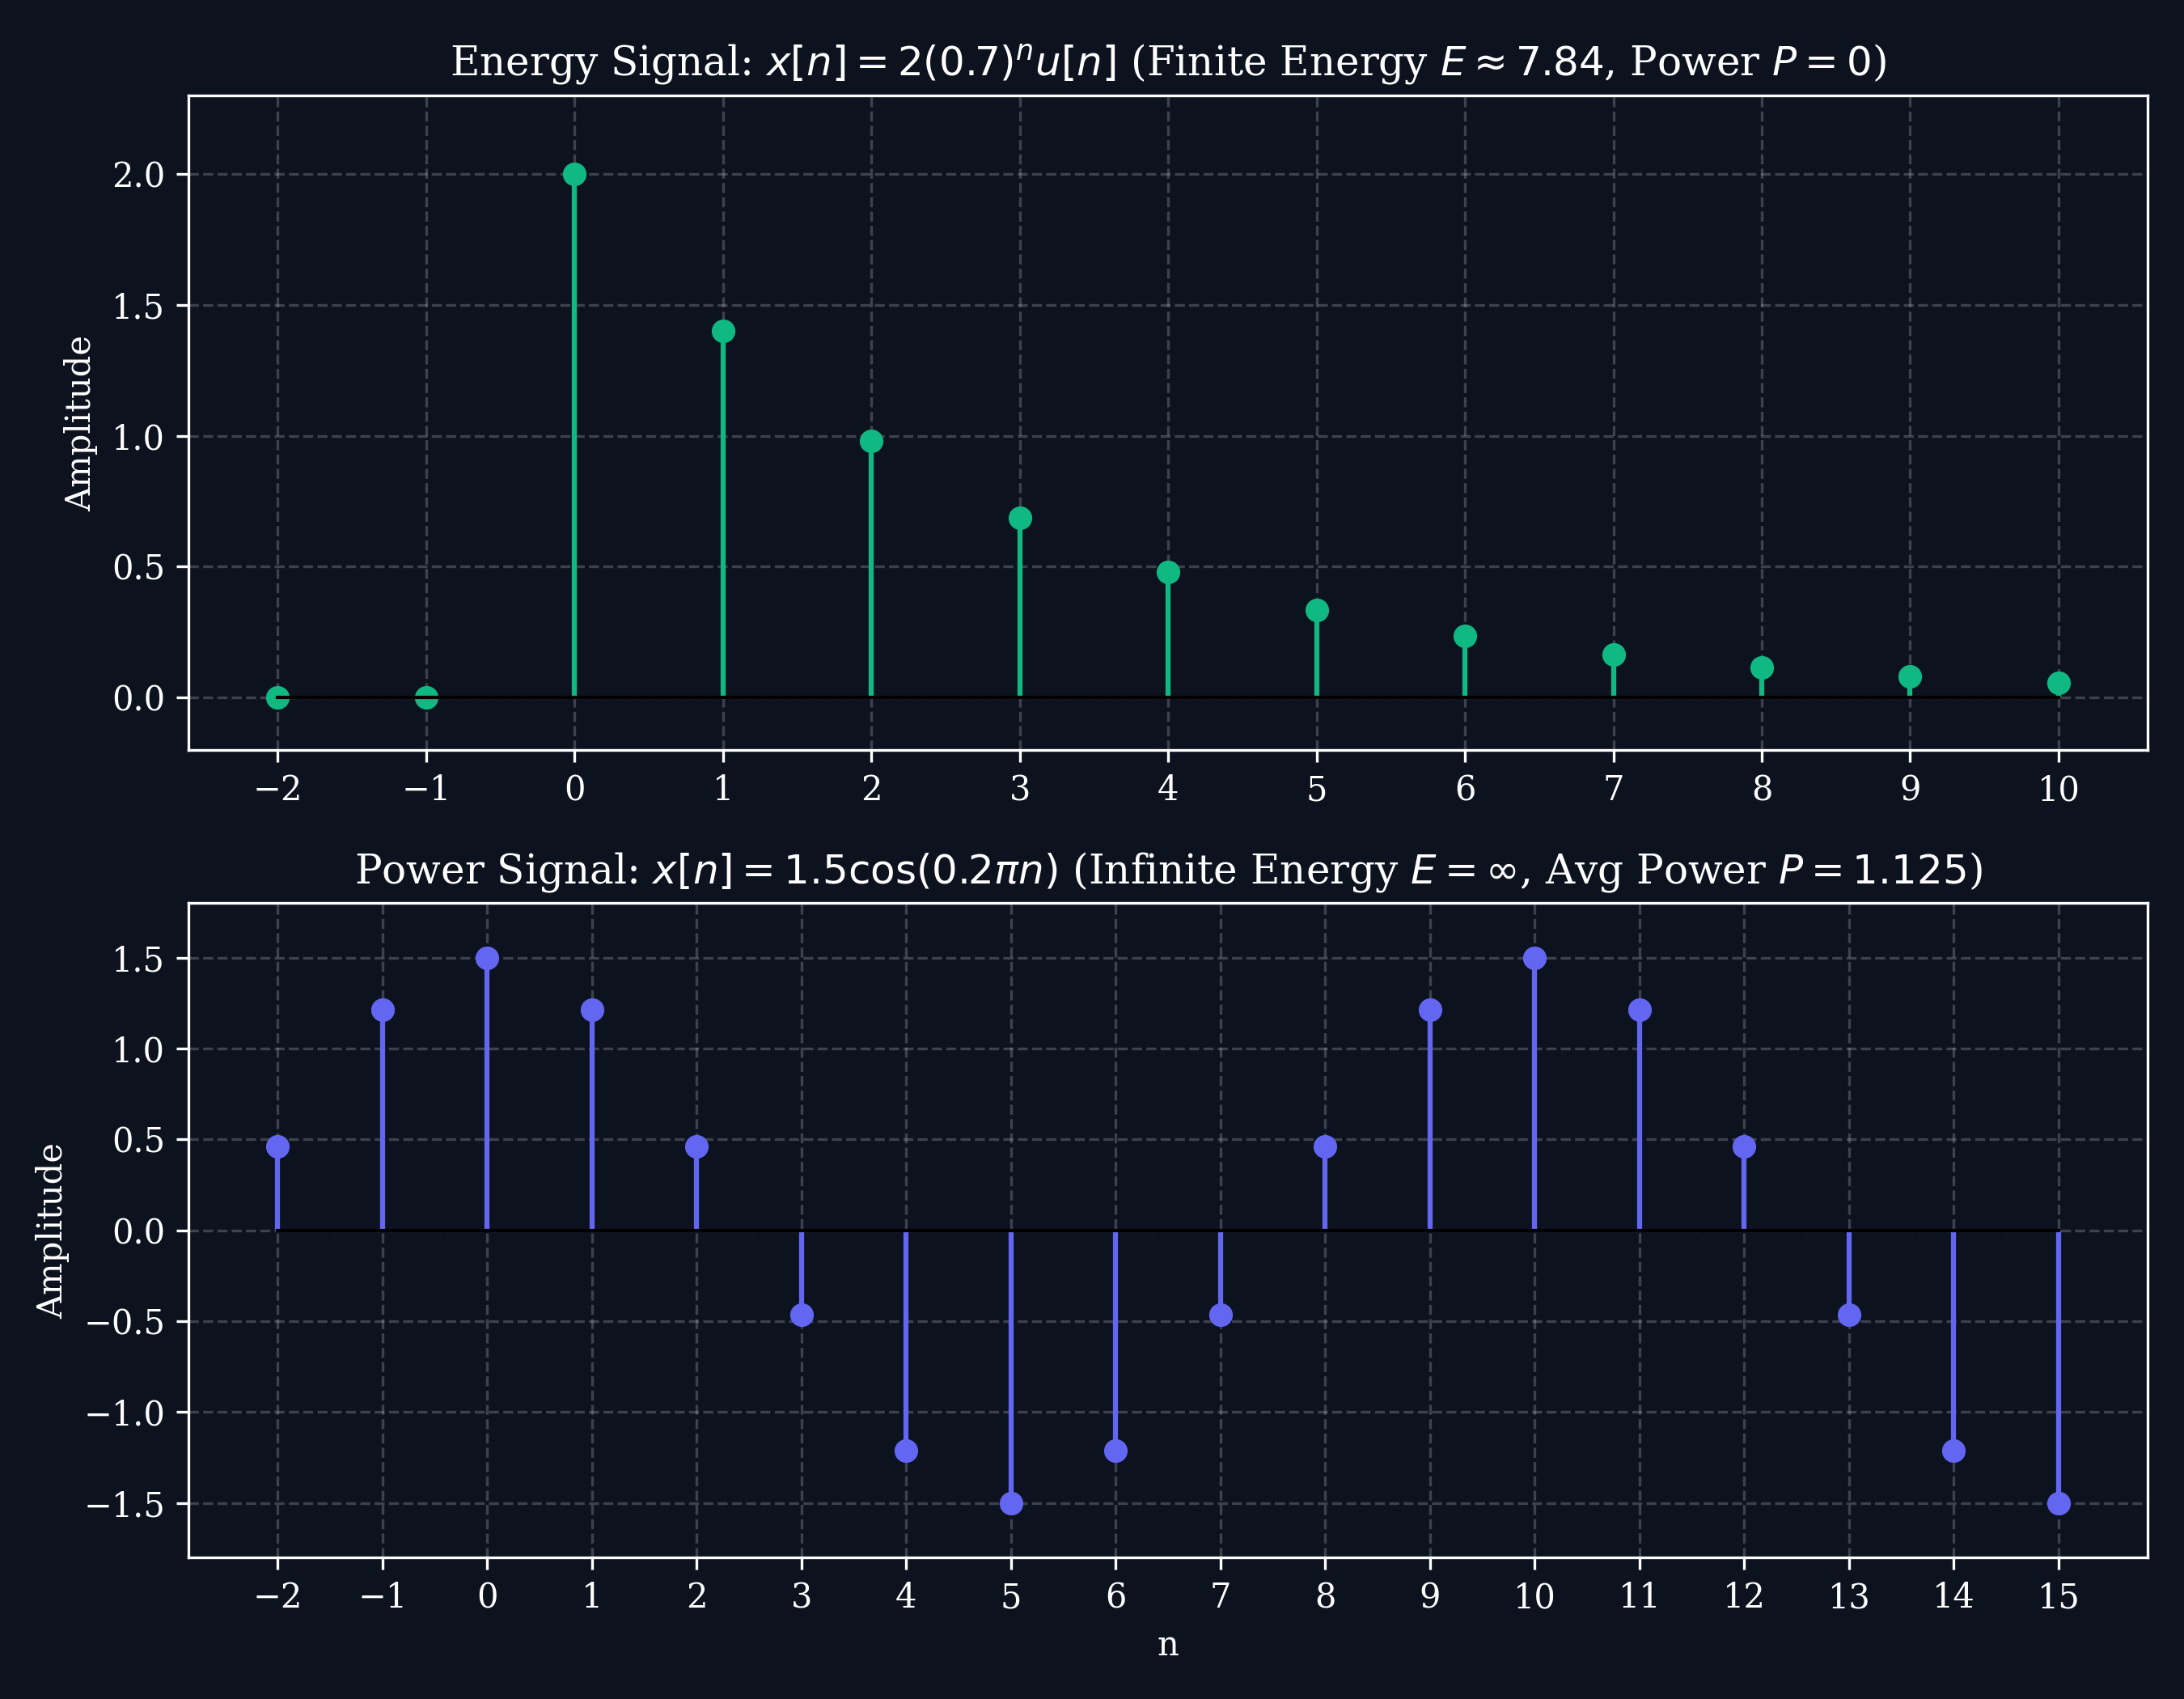
\includegraphics[width=0.75\textwidth]{images/energy_vs_power.png}
    \caption{Visual comparison of an exponential decay (Energy Signal) and a periodic sinusoid (Power Signal).}
    \label{fig:energy_vs_power}
    \end{figure}
    
    \item \textbf{Causality:}
    \begin{itemize}
        \item Causal: $x[n] = 0$ for $n < 0$.
        \item Non-causal: $x[n] \neq 0$ for some $n < 0$.
        \item Anti-causal: $x[n] = 0$ for $n \ge 0$.
    \end{itemize}
\end{enumerate}

\section{Elementary Sequences}
These fundamental sequences act as building blocks to represent complex signals.

\begin{figure}[H]
\centering
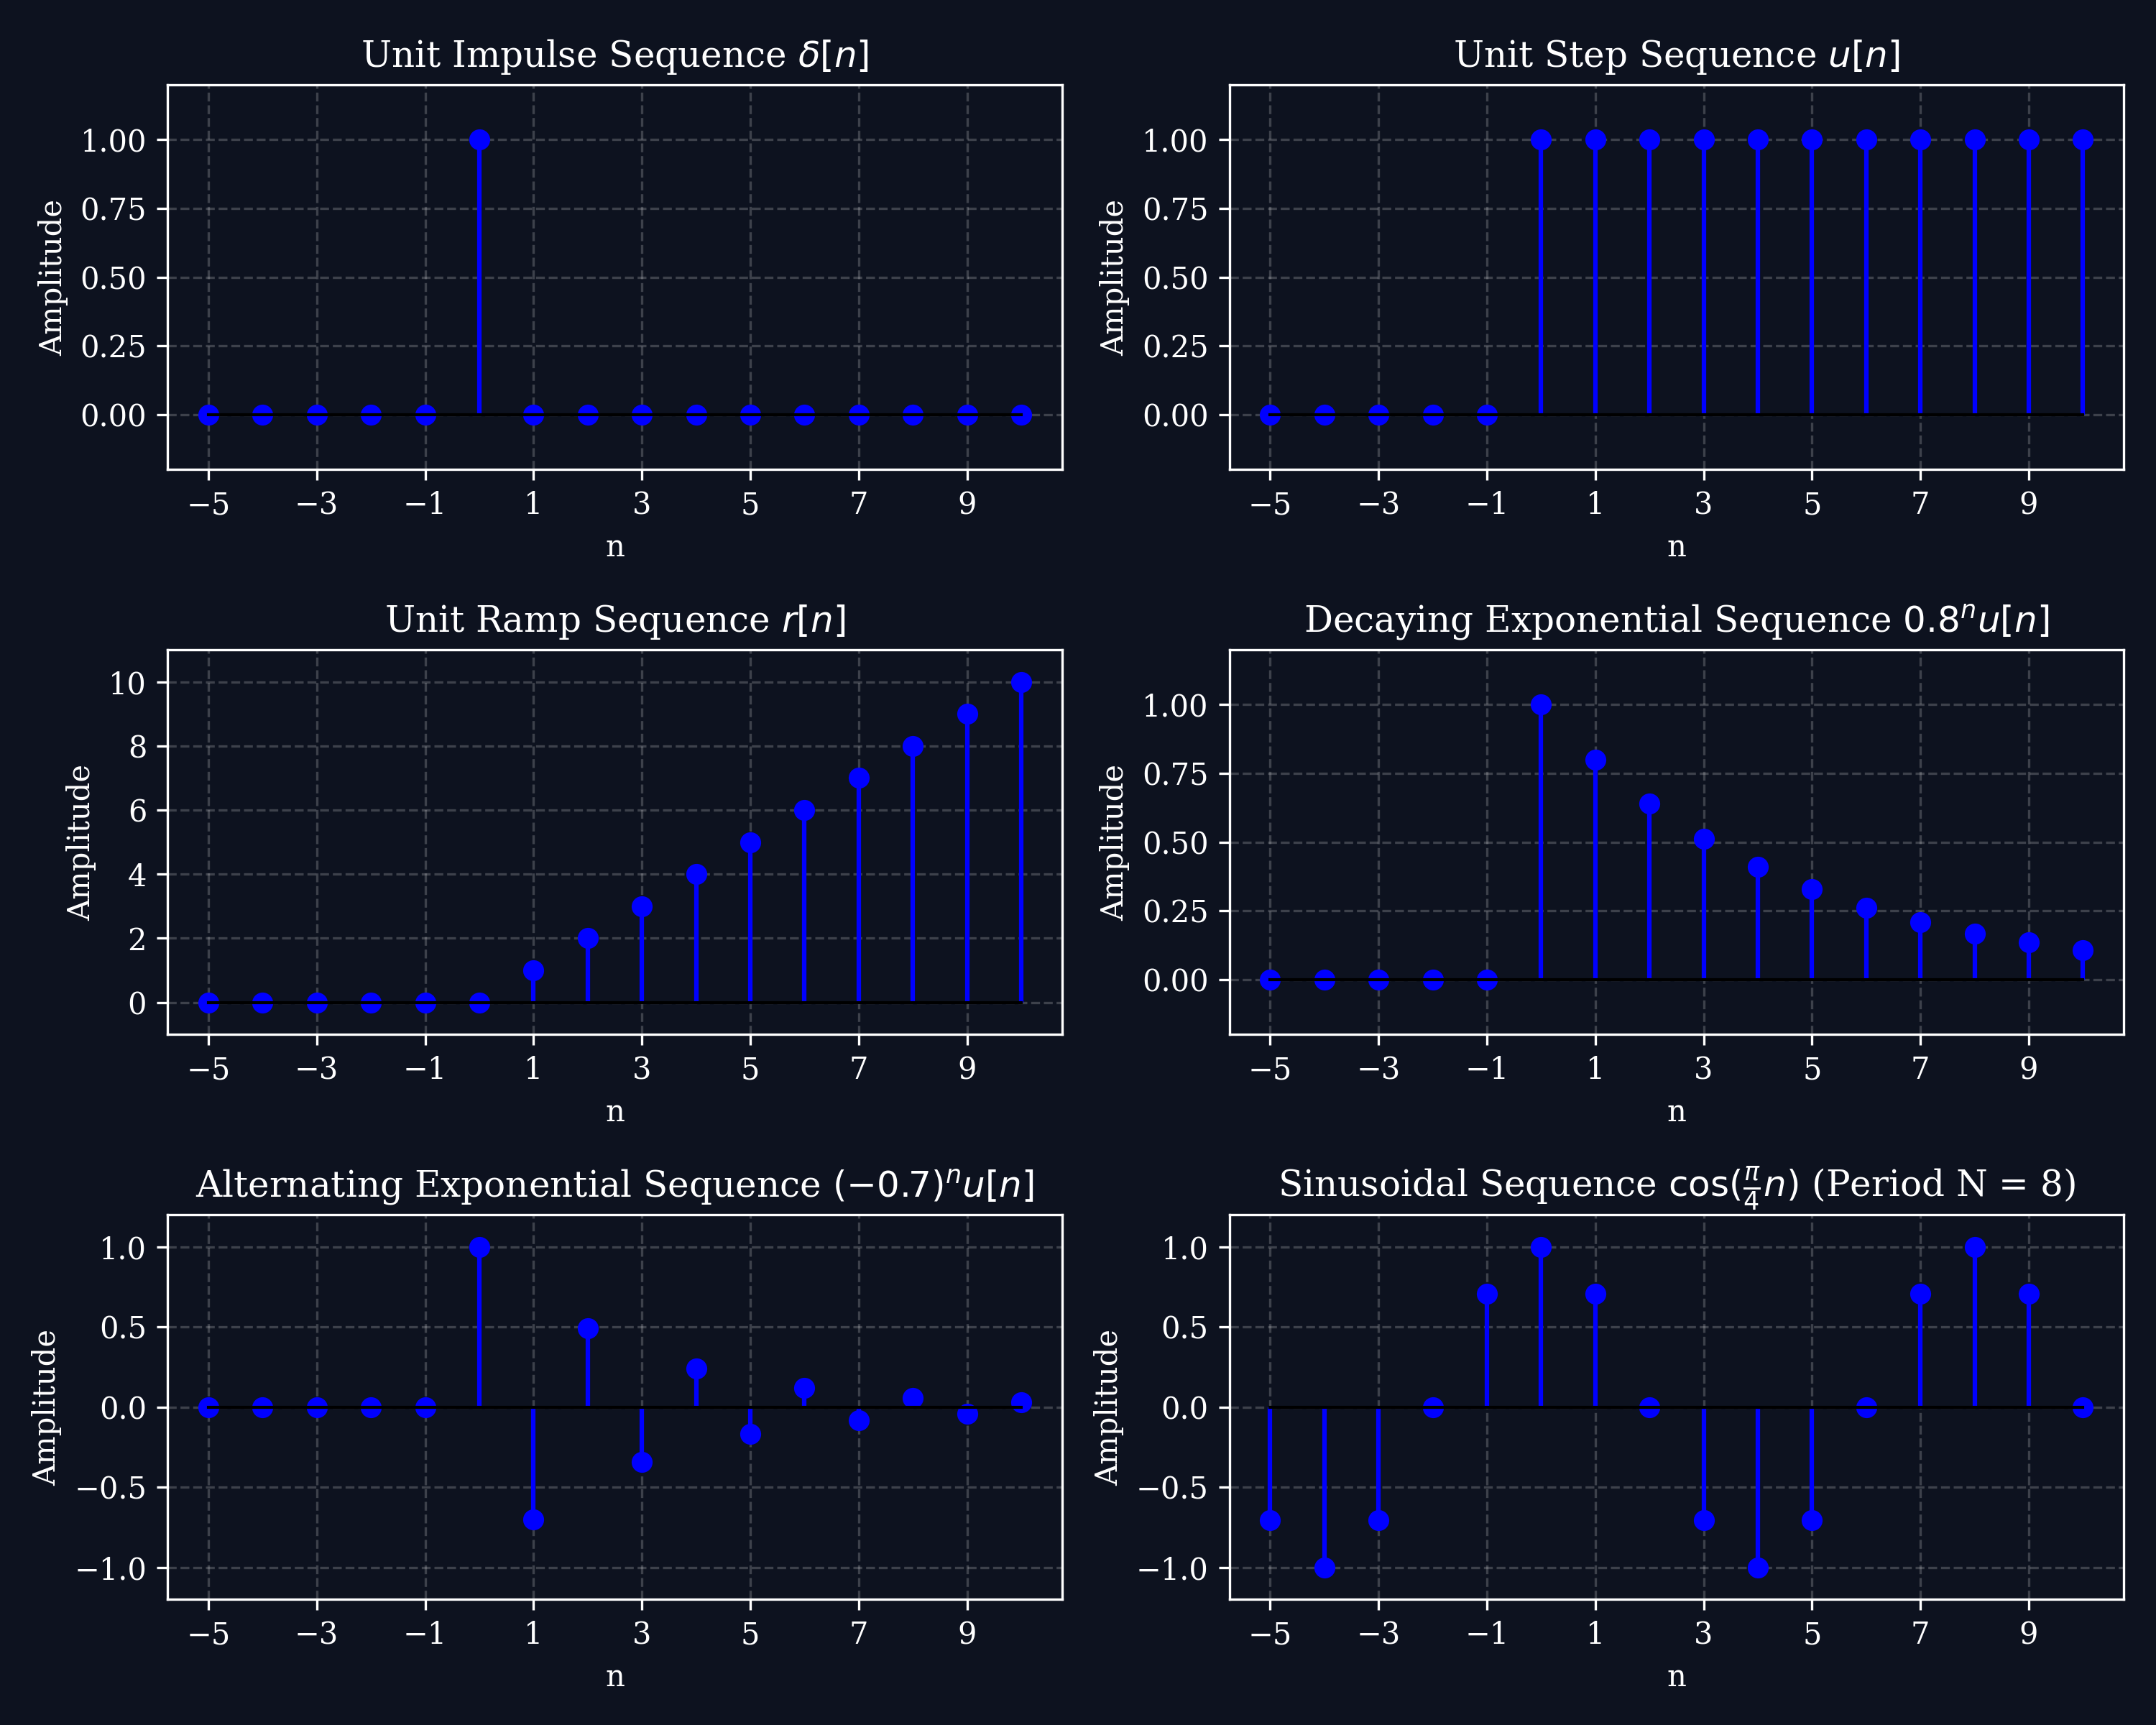
\includegraphics[width=0.9\textwidth]{images/elementary_sequences.png}
\caption{Graphical representations of elementary discrete-time sequences.}
\label{fig:elementary_sequences}
\end{figure}

\begin{itemize}
    \item \textbf{Unit Impulse $\delta[n]$:}
    \begin{equation}
    \delta[n] = \begin{cases} 1, & n = 0 \\ 0, & n \neq 0 \end{cases}
    \end{equation}
    \item \textbf{Unit Step $u[n]$:}
    \begin{equation}
    u[n] = \begin{cases} 1, & n \ge 0 \\ 0, & n < 0 \end{cases}
    \end{equation}
    \item \textbf{Unit Ramp $r[n]$:}
    \begin{equation}
    r[n] = n \cdot u[n] = \begin{cases} n, & n \ge 0 \\ 0, & n < 0 \end{cases}
    \end{equation}
    \item \textbf{Exponential Sequence $x[n] = a^n u[n]$:} (Decaying if $|a| < 1$, growing if $|a| > 1$).
    \item \textbf{Sinusoidal Sequence $x[n] = A \cos(\omega_0 n + \theta)$:} Where $\omega_0$ is the digital frequency in radians/sample.
\end{itemize}

\subsection{Operations and Properties of Signals}
Discrete-time sequences can be manipulated using basic mathematical operations:
\begin{itemize}
    \item \textbf{Time Shifting:} Shifting the signal index by an integer $n_0$:
    \begin{equation}
    y[n] = x[n - n_0]
    \end{equation}
    If $n_0 > 0$, the signal is delayed (shifted right). If $n_0 < 0$, it is advanced (shifted left).
    
    \item \textbf{Time Reversal (Folding):} Reflecting the signal about $n=0$:
    \begin{equation}
    y[n] = x[-n]
    \end{equation}
    
    \item \textbf{Time Scaling (Decimation \& Interpolation):}
    \begin{itemize}
        \item Decimation (Downsampling): $y[n] = x[D \cdot n]$, where $D \in \mathbb{Z}^+$ keeps every $D$-th sample.
        \item Interpolation (Upsampling): $y[n] = x[n/I]$ if $n$ is a multiple of $I$, and $0$ otherwise.
    \end{itemize}
    
    \item \textbf{Arithmetic Operations:} Summing ($y[n] = x_1[n] + x_2[n]$), product ($y[n] = x_1[n] \cdot x_2[n]$), or amplitude scaling ($y[n] = A \cdot x[n]$).
\end{itemize}

\subsection{Definition of a DSP System}
A \textbf{system} is defined mathematically as an operator or transformation $\mathcal{T}$ that maps an input sequence $x[n]$ to an output sequence $y[n]$:
\begin{equation}
y[n] = \mathcal{T}\{x[n]\}
\end{equation}
The digital signal processor is the physical implementation of this system. Systems are classified by these fundamental properties:
\begin{itemize}
    \item \textbf{Linearity:} Satisfies both \textbf{Additivity (Superposition)} and \textbf{Homogeneity (Scaling)}.
    \begin{enumerate}
        \item \textbf{Superposition (Additivity):}
        \begin{equation}
        \mathcal{T}\{x_1[n] + x_2[n]\} = \mathcal{T}\{x_1[n]\} + \mathcal{T}\{x_2[n]\}
        \end{equation}
        \begin{center}
        \begin{tabular}{ccccc}
        $x_1[n]$ & $\rightarrow$ & \boxed{\mathcal{T}} & $\rightarrow$ & $y_1[n]$ \\
        $x_2[n]$ & $\rightarrow$ & \boxed{\mathcal{T}} & $\rightarrow$ & $y_2[n]$ \\
        \multicolumn{5}{c}{Outputs are added: $y_A[n] = y_1[n] + y_2[n]$} \\
        \midrule
        $x_1[n] + x_2[n]$ & $\rightarrow$ & \boxed{\mathcal{T}} & $\rightarrow$ & $y_B[n] = \mathcal{T}\{x_1[n] + x_2[n]\}$
        \end{tabular}
        \\ \vspace{0.1cm}
        \textit{Linear system condition: $y_A[n] = y_B[n]$}
        \end{center}
        
        \item \textbf{Homogeneity (Scaling):}
        \begin{equation}
        \mathcal{T}\{a \cdot x[n]\} = a \cdot \mathcal{T}\{x[n]\}
        \end{equation}
        \begin{center}
        \begin{tabular}{ccccc}
        $x[n]$ & $\rightarrow$ & \boxed{\text{Scale by } a} & $\rightarrow$ & \boxed{\mathcal{T}} $\rightarrow y_A[n]$ \\
        $x[n]$ & $\rightarrow$ & \boxed{\mathcal{T}} & $\rightarrow$ & \boxed{\text{Scale by } a} $\rightarrow y_B[n]$
        \end{tabular}
        \\ \vspace{0.1cm}
        \textit{Linear system condition: $y_A[n] = y_B[n]$}
        \end{center}
    \end{enumerate}

    \textbf{Mathematical Proof: Why a Straight Line Equation is Non-Linear}\\
    Consider the system:
    \begin{equation}
    y[n] = \mathcal{T}\{x[n]\} = m \cdot x[n] + c \quad (c \neq 0)
    \end{equation}
    \begin{enumerate}
        \item \textbf{Homogeneity Check:} For input $x_1[n] = a \cdot x[n]$:
        \begin{equation}
        y_1[n] = \mathcal{T}\{a \cdot x[n]\} = m(a \cdot x[n]) + c = a m x[n] + c
        \end{equation}
        Scaling the output by $a$:
        \begin{equation}
        a \cdot y[n] = a(m \cdot x[n] + c) = a m x[n] + a c
        \end{equation}
        Since $c \neq a c$ for $c \neq 0$ (when $a \neq 1$), homogeneity is violated.
        \item \textbf{Additivity Check:} For input $x_3[n] = x_1[n] + x_2[n]$:
        \begin{equation}
        y_3[n] = m(x_1[n] + x_2[n]) + c = m x_1[n] + m x_2[n] + c
        \end{equation}
        Sum of individual outputs:
        \begin{equation}
        y_1[n] + y_2[n] = (m x_1[n] + c) + (m x_2[n] + c) = m x_1[n] + m x_2[n] + 2c
        \end{equation}
        Since $c \neq 2c$ for $c \neq 0$, additivity is violated.
    \end{enumerate}
    Thus, the straight-line affine relation $y[n] = m x[n] + c$ is a \textbf{non-linear} system.

    \item \textbf{Time-Invariance:} A time-shift of the input causes an identical time-shift of the output:
    \begin{equation}
    \mathcal{T}\{x[n - n_0]\} = y[n - n_0]
    \end{equation}
    \begin{center}
    \begin{tabular}{ccccc}
    $x[n]$ & $\rightarrow$ & \boxed{\text{Delay } n_0} & $\rightarrow$ & \boxed{\mathcal{T}} $\rightarrow y_A[n]$ \\
    $x[n]$ & $\rightarrow$ & \boxed{\mathcal{T}} & $\rightarrow$ & \boxed{\text{Delay } n_0} $\rightarrow y_B[n]$
    \end{tabular}
    \\ \vspace{0.1cm}
    \textit{Time-Invariance condition: $y_A[n] = y_B[n]$}
    \end{center}
    
    \item \textbf{Causality:} The output at index $n_0$ depends only on present and past input values ($x[n]$ for $n \le n_0$).
    
    \item \textbf{Stability:} A system is BIBO (Bounded-Input Bounded-Output) stable if every bounded input ($|x[n]| \le M_x < \infty$) produces a bounded output ($|y[n]| \le M_y < \infty$).
\end{itemize}

\section{Checkpoint \& Class Discussion Questions}
\begin{enumerate}
    \item \textbf{Q1:} Determine if $x[n] = \cos(\frac{3}{10} n)$ is periodic or aperiodic.
    \begin{itemize}
        \item \textbf{Solution:} $\omega_0 = 3/10$. Thus, $\frac{\omega_0}{2\pi} = \frac{3}{20\pi}$. Since $\pi$ is irrational, this ratio is irrational, meaning the signal is \textbf{aperiodic}.
    \end{itemize}
    \item \textbf{Q2:} Write the mathematical relationship between the unit step $u[n]$ and unit impulse $\delta[n]$.
    \begin{itemize}
        \item \textbf{Solution:} $\delta[n] = u[n] - u[n-1]$ and $u[n] = \sum_{k=0}^{\infty} \delta[n-k]$.
    \end{itemize}
\end{enumerate}

\end{document}
